\chapter{Solvers for nonlinear programming}
Once the objective function and constraints are created, the problem is passed
to the NLP solver. Popular methods are Lagrange-Newton methods, these are sequential quadratic solvers and
interior point solvers. These solvers are perhaps the most complex component used in this thesis, this chapter will cover them at high leve, as full theory is beyond the scope. A comprehensive overview of Lagrange-Newton methods is in article\cite{vanaret_implementing_2025}, where the methods are broken down into key algorithmic components and unifying framework of solvers is presented. Figure\ref{fig:wheel} shows the key algorithmic components.
\begin{figure}[H]
    \centering
    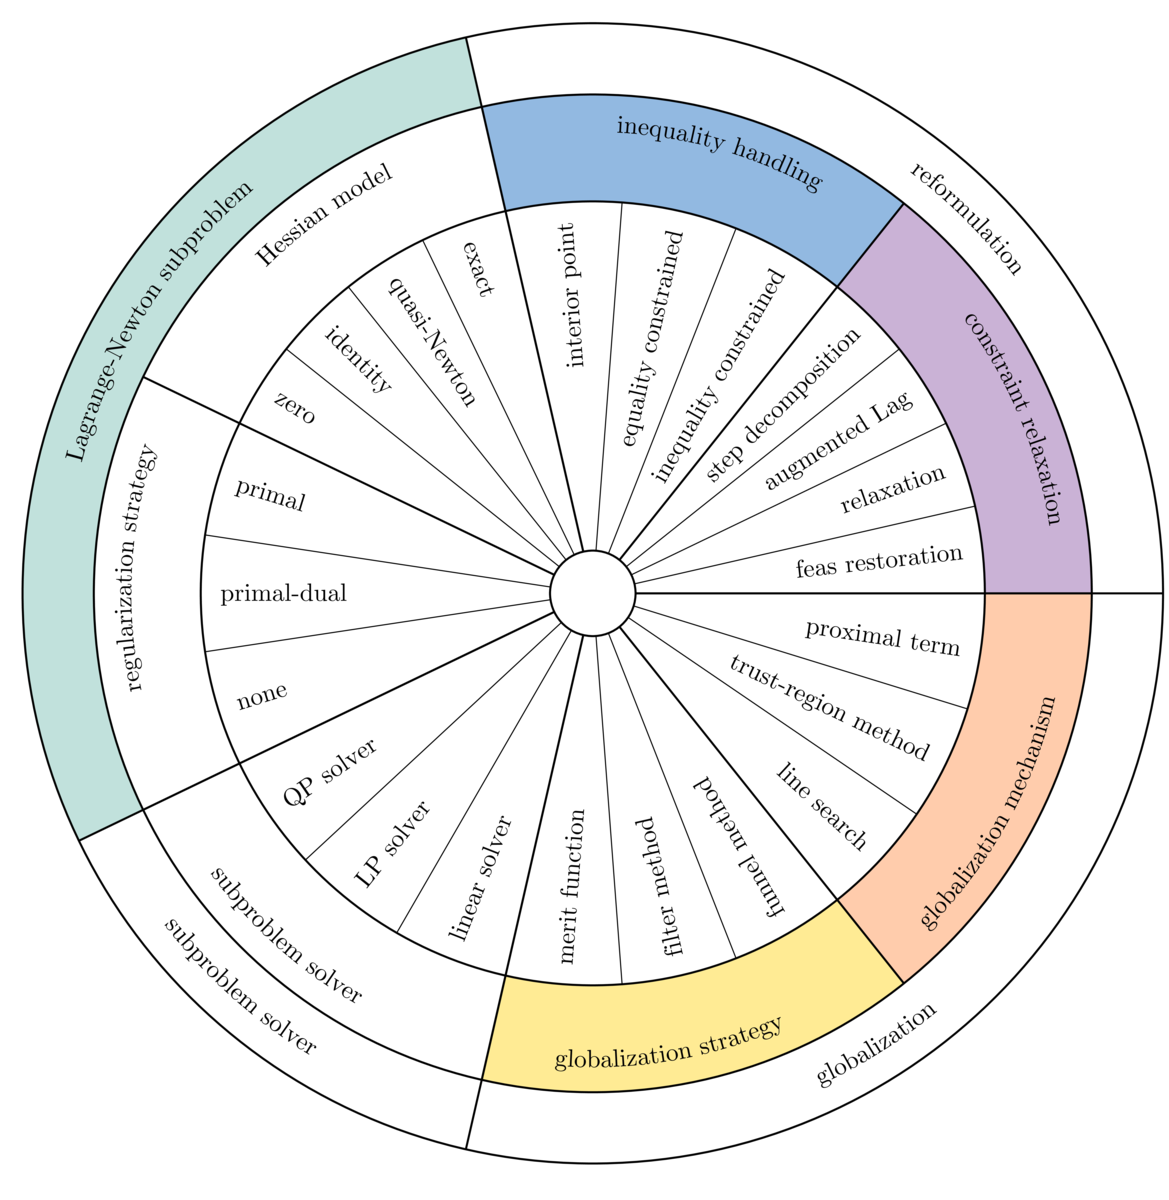
\includegraphics[width=0.8\textwidth]{figures/wheel.png}
    \caption{Unifying framework: the “wheel of strategies”\cite{vanaret_implementing_2025}}
    \label{fig:wheel}
\end{figure}
High level overview required for this thesis of Lagrange-Newton methods is in Figure \ref{fig:nlp_flowchart}. 

\begin{figure}[H]
\centering
\resizebox{\textwidth}{!}{%
\begin{tikzpicture}[
  >={Latex[length=2mm]},
  node distance=0.8cm and 0.3cm,
  every node/.style={font=\small, align=center},
  box/.style={draw, minimum height=0.8cm, inner sep=4pt},
  problem/.style={box},
  branch/.style={box, font=\small\bfseries},
  stagebox/.style={box},
  deriv/.style={box, font=\small, text width=2.2cm},
  terminal/.style={box, line width=1pt}
]

\node[problem] (nlp) {NLP problem statement};

\node[branch, below left=1.2cm and 2.2cm of nlp] (sqp) {Sequential Quadratic programming};
\node[branch, below right=1.2cm and 2.2cm of nlp] (ipm) {Interior point methods};

\node[stagebox, below=of sqp] (qp) {Quadratic model of Lagrangian,\\linearized constraints,\\QP subproblem};
\node[stagebox, below=of ipm] (bar) {Barrier problem reformulation};

\node[problem, below=3.5cm of nlp] (need) {Calucate first and second derivatives};

\node[deriv, below=1.6cm of need] (fd) {Finite\\differences};
\node[deriv, left=of fd]  (sym)  {Symbolic\\(CAS)};
\node[deriv, left=of sym] (anal) {Analytic\\(hand-coded)};
\node[deriv, right=of fd] (ad)   {Automatic differentiation};
\node[deriv, right=of ad] (qn)   {Quasi-Newton Approximation};

\node[terminal, below=4cm of need] (newton) {Assemble linear system of equations\\\textbf{Newton step}};

\draw[->] (nlp) -- (sqp);
\draw[->] (nlp) -- (ipm);
\draw[->] (sqp) -- (qp);
\draw[->] (ipm) -- (bar);
\draw[->] (qp)  -- (need);
\draw[->] (bar) -- (need);

\draw[->] (need) -- (anal);
\draw[->] (need) -- (sym);
\draw[->] (need) -- (fd);
\draw[->] (need) -- (ad);
\draw[->] (need) -- (qn);

\draw[->] (anal) -- (newton);
\draw[->] (sym)  -- (newton);
\draw[->] (fd)   -- (newton);
\draw[->] (ad)   -- (newton);
\draw[->] (qn)   -- (newton);

\end{tikzpicture}}
\caption{NLP solution flow: problem statement $\to$ solver family (SQP / IPM) $\to$ derivative computation $\to$ assembled Newton step.}
\label{fig:nlp_flowchart}
\end{figure}



\section{Nonlinear programming}

General NLP problems can be written as:
\begin{equation}
    \begin{aligned}
        \min_{\mathbf{x} \in \mathbb{R}^n} \quad & f(\mathbf{x})                 \\
        \text{s.t.} \quad                        & \mathbf{h}(\mathbf{x}) = 0    \\
                                                 & \mathbf{g}(\mathbf{x}) \leq 0
    \end{aligned}
    \label{eq:general_nlp}
\end{equation}

Here $\mathbf{x} \in \mathbb{R}^n$ is the decision-variable vector, $f : \mathbb{R}^n \to \mathbb{R}$ is the scalar objective, $\mathbf{h} : \mathbb{R}^n \to \mathbb{R}^m$ stacks the $m$ equality constraints, and $\mathbf{g} : \mathbb{R}^n \to \mathbb{R}^p$ stacks the $p$ inequality constraints. In the lap-time setting $\mathbf{x}$ holds the discretised states and controls, $f$ is total lap time, $\mathbf{h}$ enforces vehicle dynamics and boundary conditions, and $\mathbf{g}$ enforces track limits, tire friction circle and actuator bounds.

\subsection{KKT conditions}
KKT condiitons are the conditions of optimality, if satisfied the point is local optimum.
alpha and omega of nolinear programming, lord praise the KKT conditions.

\begin{equation}
    \begin{aligned}
        \nabla f(\mathbf{x}) + \sum_{i=1}^{m} \lambda_i \nabla h_i(\mathbf{x}) + \sum_{i=1}^{p} \mu_i \nabla g_i(\mathbf{x}) & = 0                            \\
        \mathbf{h}(\mathbf{x})                                                                                               & = \mathbf{0}                   \\
        \mathbf{g}(\mathbf{x})                                                                                               & \leq \mathbf{0}                \\
        \mu_i                                                                                                                & \geq 0, \quad i = 1, \ldots, p \\
        \mu_i g_i(\mathbf{x})                                                                                                & = 0, \quad i = 1, \ldots, p
    \end{aligned}
\end{equation}


%\begin{equation}
%    \begin{pmatrix}
%        \nabla^2 \mathcal{L} & A^T \\
%        A                    & 0
%    \end{pmatrix}
%    \begin{pmatrix}
%        -\Delta x \\
%        \lambda
%    \end{pmatrix}
%    =
%    \begin{pmatrix}
%        \nabla f(x) \\
%        c(x)
%    \end{pmatrix}
%\end{equation}

\section{Interior point methods: IPOPT, MadNLP}
\label{sec:interior_point}

Interior point solvers or barrier solvers work by reformulating the NLP into a
barrier problem at each step and solving a sequence of these barrier problems, with decreasing
barrier parameter. Solver used in this thesis is IPOPT \cite{wachter_implementation_2006} and MadNLP\cite{shin2024accelerating}.

\subsection{Barrier problem formulation}
\label{subsec:barrier_problem_formulation}
There are multiple ways to transform NLP in to barrier problem, this section
will briefly describe how IPOPT does it.
IPOPT article~\cite{wachter_implementation_2006} Describes how to transform generic
NLP into form~\ref{eq:barrier_problem} 

\begin{equation}
    \begin{aligned}
        \min_{\mathbf{x} \in \mathbb{R}^n} \quad & \phi_\mu(\mathbf{x}) := f(\mathbf{x}) - \mu \sum_{i=1}^{n} \ln(x_i^{(i)}) \\
        \text{s.t.} \quad                        & c(\mathbf{x}) = 0
    \end{aligned}
    \label{eq:barrier_problem}
\end{equation}

 The Lagrangian of the barrier problem is defined as
\begin{equation}
    \mathcal{L}(\mathbf{x}, \lambda, z) := f(\mathbf{x}) + c(\mathbf{x})^\top \lambda - z.
    \label{eq:lagrangian_barrier}
\end{equation}
Then barrier problem is further transformed into set of linear equations, a KKT linear system, that
computes the Newton step:
\begin{equation}
    \begin{bmatrix}
        W_k   & A_k & -I  \\
        A_k^T & 0   & 0   \\
        Z_k   & 0   & X_k
    \end{bmatrix}
    \begin{bmatrix}
        d_x^k       \\
        d_\lambda^k \\
        d_z^k
    \end{bmatrix}
    = -
    \begin{bmatrix}
        \nabla f(x_k) + A_k \lambda_k - z_k \\
        c(x_k)                              \\
        X_k Z_k e - \mu_j e
    \end{bmatrix}.
\end{equation}
Here $W_k = \nabla^2 \mathcal{L}(x_k, \lambda_k, z_k)$ is the Hessian of the Lagrangian, $A_k$ is the Jacobian of the equality constraints $c(x)$ and $\nabla f(x_k)$ is the gradient of the objective. The unknowns $d_x^k$, $d_\lambda^k$ and $d_z^k$ are the Newton steps in the primal variables, equality multipliers and bound multipliers; $\mu_j$ is the barrier parameter, which is driven to zero across outer iterations.

There are numerous commercial and free algorithms to solve this. For smaller
systems it is LU decomposition, but for larger sparse problems a dedicated
solver is a must. IPOPT is most commonly used with MUMPS \cite{MUMPS:1} solver
which is free. There are several linear commercial solvers, Harwell Subroutine
Library(HSL) offers ma27 ma87 ma97 \cite{hsl2011collection}.Panua technologies offers PARDISO solver
\cite{pardiso}. Harwell Subroutine Library solvers are available free for
academic usage and PARDISO solver is available free for academic usage. Latter solvers run on CPU, Nvidia has linear solver CuDSS\cite{nvidia_cudss} which runs on GPU.
Linear solver are capable of multithreading on CPU, which needs to be explicitly
turned on. 

\section{Sequential quadratic programming}
Sequential quadratic programming is less commonly used for offline trajectory optimisation, usage of IPOPT prevails.

\section{Calculation of derivatives}
Major complication of many Lagrange-Newton methods is that they require gradient of the objective function, Jacobian of the constraints and Hessian of the Lagrangian to compute the Newton step. Computing these derivatives can be time intensive. The most universal method is finite differences, which means evaluating the function around the current point and estimating the derivative, this works even for a black box model, but the derivatives are not exact. When the model is available, symbolic differentiation can be used, however, the full symbolic expression is often too large to be evaluated effectively due to repeated chain and product rules. Automatic differentiation aims to solve the problems of previous methods, by applying the chain rule to the elementary operations of a function. A comprehensive review of automatic differentiation is given in~\cite{cortildBriefReviewAutomatic2023}.


\section{Scaling and matrix conditioning}
Common pitfall of nonlinear programming is poor scaling. This happens when the
solver encounters variables, that are orders of magnitude apart, for example
motor force in thousands of newton and heading angle in radians. This happens,
because at the core of nonlinear programming solver is a linear solver WROOOOONG elipsa zoptimalziace to inka ukazuje
(MUMPS,MA97,PARDISO,...), that has to do matrix factorization every iteration,
to solve KKT linear system. If this linear system is ill conditioned due to
improper scaling, the factorization may be imprecise and search direction
corrupted.

Another thing which led to issues is constraints qualification. Linear
indpendence constiant qualification requires gradients of the active
constraints to be linearly independent. If it is violated, the jacobian of the constraints is
rank deficient and linear solve may fails

\section{sparsity}
Sparsity is good, sparsity means matrix hessians and jacobians with many zeros
also sparsisty in constraints, that means not having super very long expression
with many terms in constraint. I guess it is beacause deriavtive is difficult
then and can lead solver in wrong direction or take small stages. Therefore
using more decison variables to define same problem can actually lead to faster
computation \cite{julia_discourse_ipopt_hessian}. Certain solvers can exploit
the sprasity strcuture, such as FATROP\cite{vanroyeFATROPFastConstrained2023}.
In source \cite{jorisgillisIPOPTSteroidsFatrop2024} Joris gillis a casadi
developer compares IPOPT to FATROP, with \textbf{FATROP being 33 times faster
    on a trajecotry optimisation problem.}

Also \cite{betts} describes how sprasity structure helps with afster hessian
aprprixmiation for using finite difference??? secant method.

\section{Initialization}
NLP solvers require initial guess for all decision variables, to start solving.
For this problem initial guess is obtained driving the vehicle on given track.
PD controller is used to keep the car on the centerline and P controller is
used to keep velocity at 5m/s. In general, it is possible to initialize all
variables at zero, but with large scale nonlinear programming this approach is
not used. For this problem initialization with zeros leads to singularity in
equation \ref{time2path} and is not possible at all. must be ineitialzied
otherwise very baaaadt?

\section{Global and local optimums}
This optimization problem is generally non convex, therefore any local optimum
does not guarantee global optimum.Commonly used NLP solvers, like IPOPT
guarantee only local optimums and not global ones. Good initization is basis
for finding a local optimum close to the global optimum. Source?????